\documentclass[10pt]{beamer}

% Beamer style
%\usetheme[secheader]{Madrid}
% \usetheme{CambridgeUS}
\useoutertheme{infolines}
\usecolortheme[rgb={0.65,0.15,0.25}]{structure}
% \usefonttheme[onlymath]{serif}
\beamertemplatenavigationsymbolsempty
%\AtBeginSubsection

% Packages
%\usepackage[french]{babel}
\usepackage[latin1]{inputenc}
\usepackage{color}
\usepackage{xspace}
%\usepackage{dsfont, stmaryrd}
\usepackage{amsmath, amsfonts, amssymb}
\usepackage{epsfig}
\usepackage{url}
\usepackage{/home/robin/LATEX/Biblio/astats}
%\usepackage[all]{xy}
\usepackage{graphicx}

% Commands
\definecolor{darkred}{rgb}{0.65,0.15,0.25}
%\newcommand{\emphase}[1]{\textcolor{darkred}{#1}}
\newcommand{\emphase}[1]{{#1}}
\newcommand{\paragraph}[1]{\textcolor{darkred}{#1}}
\newcommand{\refer}[1]{{\footnotesize{\textcolor{gray}{{\cite{#1}}}}}}
\newcommand{\Refer}[1]{{\footnotesize{\textcolor{gray}{{#1}}}}}
\renewcommand{\newblock}{}

% Symbols
\newcommand{\Abf}{{\bf A}}
\newcommand{\Beta}{\text{B}}
\newcommand{\Bcal}{\mathcal{B}}
\newcommand{\BIC}{\text{BIC}}
\newcommand{\Ccal}{\mathcal{C}}
\newcommand{\dd}{\text{~d}}
\newcommand{\dbf}{{\bf d}}
\newcommand{\Dcal}{\mathcal{D}}
\newcommand{\Esp}{\mathbb{E}}
\newcommand{\Ebf}{{\bf E}}
\newcommand{\Ecal}{\mathcal{E}}
\newcommand{\Gcal}{\mathcal{G}}
\newcommand{\Gam}{\mathcal{G}\text{am}}
\newcommand{\Hcal}{\mathcal{H}}
\newcommand{\Ibb}{\mathbb{I}}
\newcommand{\Ibf}{{\bf I}}
\newcommand{\ICL}{\text{ICL}}
\newcommand{\Cov}{\mathbb{C}\text{ov}}
\newcommand{\Corr}{\mathbb{C}\text{orr}}
\newcommand{\Var}{\mathbb{V}}
\newcommand{\Vsf}{\mathsf{V}}
\newcommand{\pen}{\text{pen}}
\newcommand{\Fcal}{\mathcal{F}}
\newcommand{\Hbf}{{\bf H}}
\newcommand{\Jcal}{\mathcal{J}}
\newcommand{\Kbf}{{\bf K}}
\newcommand{\Lcal}{\mathcal{L}}
\newcommand{\Mcal}{\mathcal{M}}
\newcommand{\mbf}{{\bf m}}
\newcommand{\mum}{\mu(\mbf)}
\newcommand{\Ncal}{\mathcal{N}}
\newcommand{\Nbf}{{\bf N}}
\newcommand{\Nm}{N(\mbf)}
\newcommand{\Ocal}{\mathcal{O}}
\newcommand{\Obf}{{\bf 0}}
\newcommand{\Omegas}{\underset{s}{\Omega}}
\newcommand{\Pbf}{{\bf P}}
\newcommand{\Pt}{\widetilde{P}}
\newcommand{\Pcal}{\mathcal{P}}
\newcommand{\Qcal}{\mathcal{Q}}
\newcommand{\Rbb}{\mathbb{R}}
\newcommand{\Rcal}{\mathcal{R}}
\newcommand{\Scal}{\mathcal{S}}
\newcommand{\Ucal}{\mathcal{U}}
\newcommand{\Vcal}{\mathcal{V}}
\newcommand{\BP}{\text{BP}}
\newcommand{\EM}{\text{EM}}
\newcommand{\VEM}{\text{VEM}}
\newcommand{\VBEM}{\text{VBEM}}
\newcommand{\cst}{\text{cst}}
\newcommand{\obs}{\text{obs}}
\newcommand{\ra}{\emphase{\mathversion{bold}{$\rightarrow$}~}}
%\newcommand{\transp}{\text{{\tiny $\top$}}}
\newcommand{\transp}{\text{{\tiny \mathversion{bold}{$\top$}}}}
\newcommand{\logit}{\text{logit}\xspace}

% Directory
\newcommand{\figmixt}{/home/robin/ENSEIGN/COURS/MELANGE}
\newcommand{\figbma}{/home/robin/RECHERCHE/RUPTURES/MELANGE/Exemples/Grippe}
\newcommand{\fignet}{../FIGURES}
\newcommand{\figeco}{/home/robin/RECHERCHE/ECOLOGIE/EXPOSES/FIGURES}
%\newcommand{\figmotif}{/home/robin/RECHERCHE/RESEAUX/Motifs/FIGURES}


%====================================================================
%====================================================================

%====================================================================
%====================================================================
\begin{document}
%====================================================================
%====================================================================

%====================================================================
\title[Network analysis using $W$-graphs]{Network analysis with the $W$-graph model \\ {\large (via the Stochastic Block Model)}}

\author[S. Robin]{S. Robin \\ ~\\
  Joint work with P. Latouche and S. Ouadah}

\institute[INRA / AgroParisTech]{INRA / AgroParisTech \\
  \vspace{-.1\textwidth}
  \begin{tabular}{ccccc}
    
\includegraphics[height=.3\textheight]{\fignet/LogoINRA-Couleur} & 
    \hspace{.02\textheight} &
    
\includegraphics[height=.08\textheight]{\fignet/logagroptechsolo} & 
    \hspace{.02\textheight} &
    
\includegraphics[height=.09\textheight]{\fignet/logo-ssb}
    \\ 
  \end{tabular} \\
  \bigskip
  }

\date[EMS, Amsterdam, 2015]{Vrije Univ., July 2015, Amsterdam}

%====================================================================
%====================================================================
\maketitle
%====================================================================

% %====================================================================
% \frame{\frametitle{Outline}
%   \tableofcontents
%   }
% %====================================================================

%====================================================================
%====================================================================
\section{Modeling heterogeneity in interaction networks}
\frame{\frametitle{Outline} \tableofcontents[currentsection]}
%====================================================================

%====================================================================
\subsection*{Heterogeneity in observed networks}
%====================================================================
\frame{\frametitle{Heterogeneity in observed networks} 

  Networks describe interactions between entities: genes, proteins, individuals, species... \\
  ~\\
  Observed networks display heterogeneous topologies, that one would like to decipher and better understand. \\
  ~\\

  \pause
    \begin{tabular}{ll}
    %\hspace{-.02\textwidth}
    \begin{tabular}{p{.5\textwidth}}
      \paragraph{Dolphine social network.} \\
      \includegraphics[width=.4\textwidth]{../FIGURES/NeG04-Fig11} \\
      \refer{NeG04} \\ ~\\ ~\\ ~\\
    \end{tabular}
    & 
    \hspace{-.1\textwidth}
    \begin{tabular}{p{.5\textwidth}}
      \paragraph{{\sl H. pylori} Protein-protein interaction network.} \\
      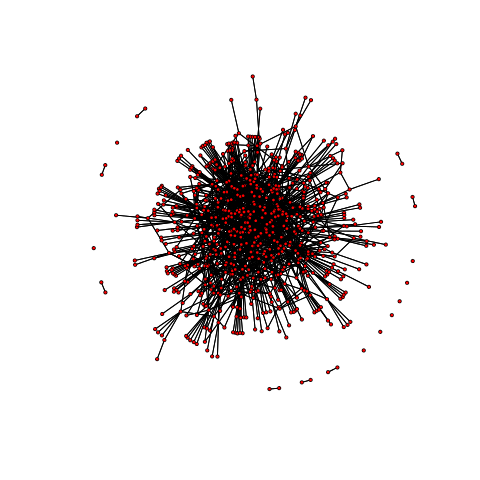
\includegraphics[width=.4\textwidth]{../FIGURES/Hpylo20060402-graph}
    \end{tabular} 
  \end{tabular} 
  }

%====================================================================
\subsection*{Latent space graph models}
%====================================================================
\frame{\frametitle{Latent space graph models}

  \paragraph{Heterogeneous means ... not homogeneous,} that is to say:  different from an Erd�s-Renyi (ER) graph 
  $$
  Y_{ij} = \Ibb\{i \sim j\}, \qquad
  (Y_{ij})_{1 \leq i < j \leq n} \text{ iid, } \qquad 
  Y_{ij} \sim \Bcal(p).
  $$

  \bigskip \pause
  \paragraph{Latent variables} capture some underlying structure of a network. The general setting for binary graphs is \refer{BJR07}: %\pause
  \begin{itemize}
   \item   \emphase{A latent (unobserved) variable $Z_i$} is associated with each node:
  $$
  \{Z_i\} \text{ iid } \sim \pi 
  $$
  \item 
  Edges \emphase{$Y_{ij} = \Ibb\{i \sim j\}$ are independent conditionally} to the $Z_i$'s:
  $$
  \{Y_{ij}\} \text{ independent } | \{Z_i\}: \Pr\{Y_{ij} = 1\} = \gamma(Z_i, Z_j)
  $$
  \end{itemize}
  
  \bigskip
  \paragraph{Review on such models:} \Refer{Matias and R. (2014)}\nocite{MaR14}.
}

%====================================================================
\subsection*{Stochastic block model}
%====================================================================
%====================================================================
\frame{\frametitle{Stochastic Block Model (SBM)}

  \begin{tabular}{cc}
    \hspace{-.02\textwidth}
    \begin{tabular}{p{.5\textwidth}}
      \onslide+<1->{
	\paragraph{A mixture model for random graphs.}} \refer{NoS01}
      \onslide+<2->{
	\begin{itemize}
        \item Consider $n$ nodes ($i = 1..n$); \\ ~ } 
        \onslide+<3->{
        \item $Z_i = $ unobserved label of node $i$:
          $$
          \{Z_i\} \text{ iid } \sim \Mcal(1; \pi)
          $$
          $\pi = (\pi_1, ... \pi_K)$; \\ ~ } 
        \onslide+<4->{
        \item Edge $Y_{ij}$ depends on the labels:
          $\{Y_{ij}\}$ independent given $\{Z_i\}$,
          $$
          \Pr\{Y_{ij} = 1\} = \gamma(Z_i, Z_j)
          $$}
      \end{itemize}
    \end{tabular}
    & 
    \hspace{-.02\textwidth}
    \begin{tabular}{p{.5\textwidth}}
      \vspace{.02\textheight}
      \begin{overprint}
        \onslide<2>
        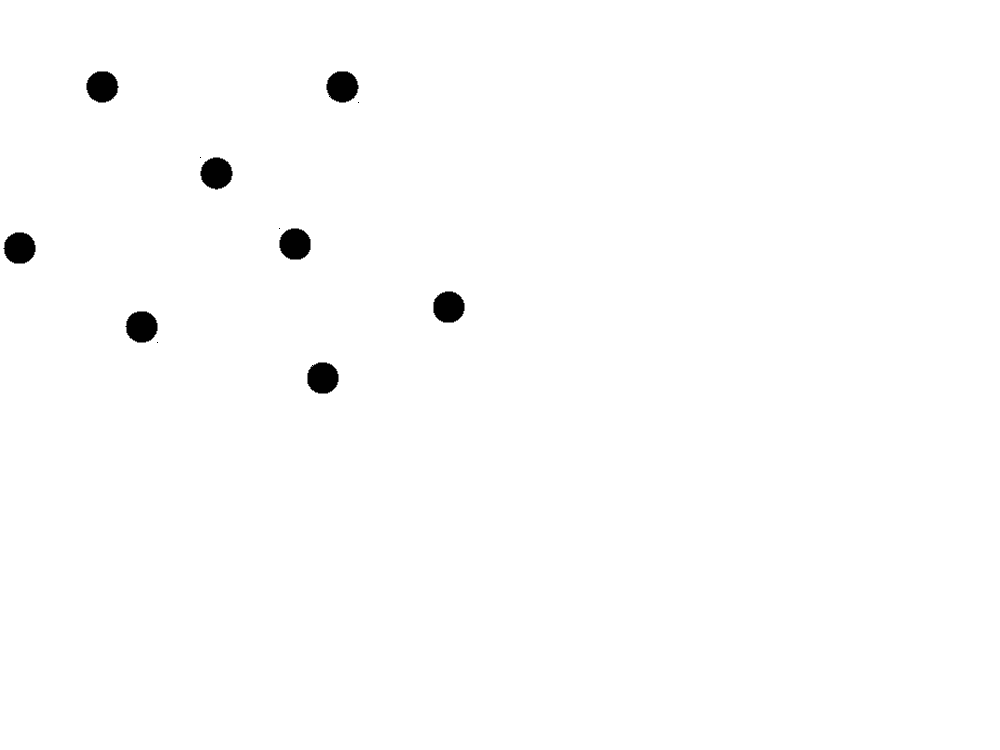
\includegraphics[width=.75\textwidth]{\fignet/FigSBM-Model-1}    
        \onslide<3>
        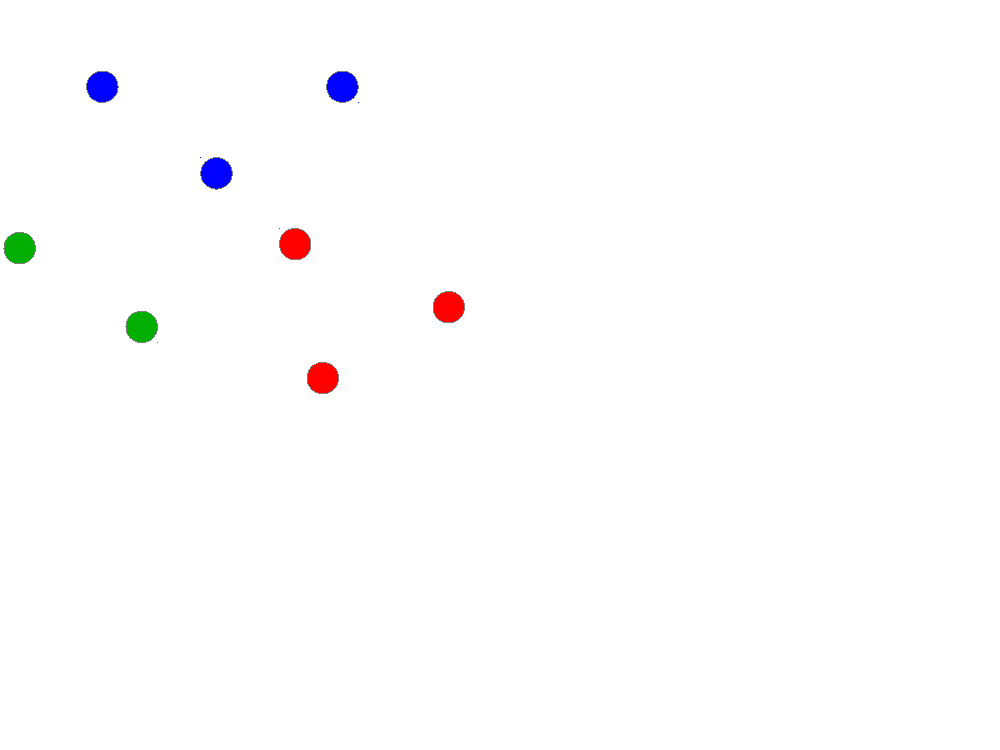
\includegraphics[width=.75\textwidth]{\fignet/FigSBM-Model-2}    
        \onslide<4>
        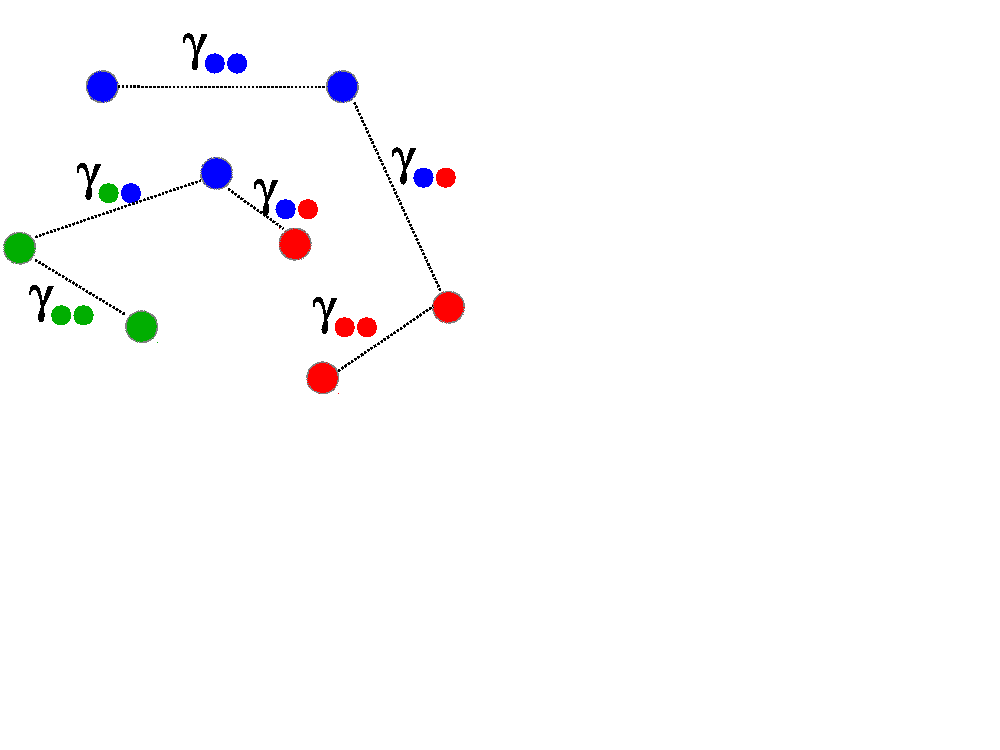
\includegraphics[width=.75\textwidth]{\fignet/FigSBM-Model-3}    
        \onslide<5>
        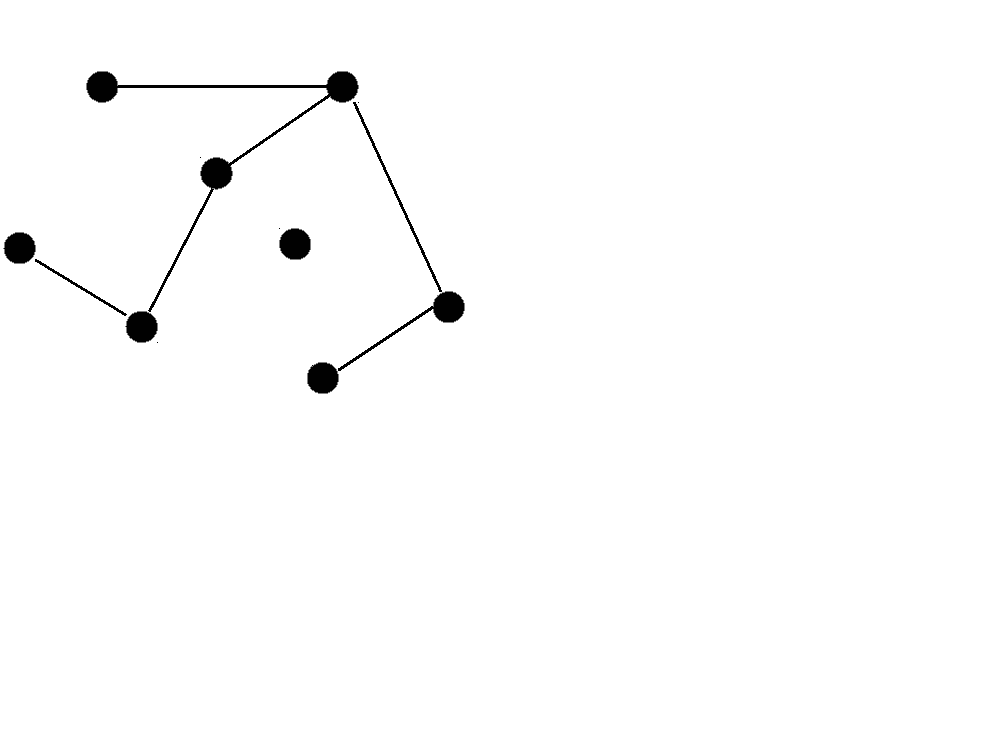
\includegraphics[width=.75\textwidth]{\fignet/FigSBM-Model-5}    
      \end{overprint}
    \end{tabular}
  \end{tabular} \\
  \vspace{-.1\textheight}
  \onslide+<4->{\paragraph{Remark:} $K = 1$ \ra ER model}
  }

%====================================================================
\subsection*{$W$-graph / graphon model}
%====================================================================
%====================================================================
\frame{ \frametitle{$W$-graph model}

  \begin{tabular}{cc}
    \hspace{-.02\textwidth}
    \begin{tabular}{p{.5\textwidth}}
	 Latent variables:
	 $$
	 (Z_i) \text{ iid } \sim \Ucal_{[0, 1]},
	 $$ ~\\
	 Graphon function $\gamma$:
	 $$
	 \gamma(z, z'): [0, 1]^2 \rightarrow [0, 1]
	 $$ ~\\    
	 Edges:
	 $$
	 \Pr\{Y_{ij} = 1\} = \gamma(Z_i, Z_j)
	 $$    
	 \end{tabular}
    & 
    \hspace{-.1\textwidth}
    \begin{tabular}{p{.5\textwidth}}
	 Graphon function $\gamma(z, z')$ \\
      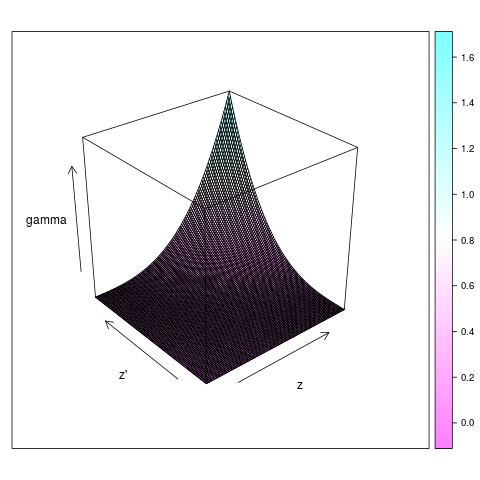
\includegraphics[width=.5\textwidth]{../FIGURES/FigCLADAG-W-graphon} \\
    \end{tabular}
  \end{tabular}
  
 }

%====================================================================
\frame{\frametitle{Interpreting the graphon function}

  The graphon function provides a global picture of the network's topology.

  \bigskip \bigskip 
  \centerline{
  \begin{tabular}{ccc}
  'Scale free' & Community & Small world \\
  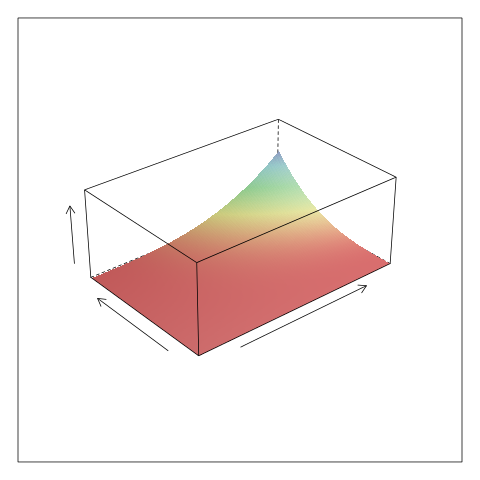
\includegraphics[width=.3\textwidth]{../FIGURES/EDD-ScaleFreeTrueGraphon} &
  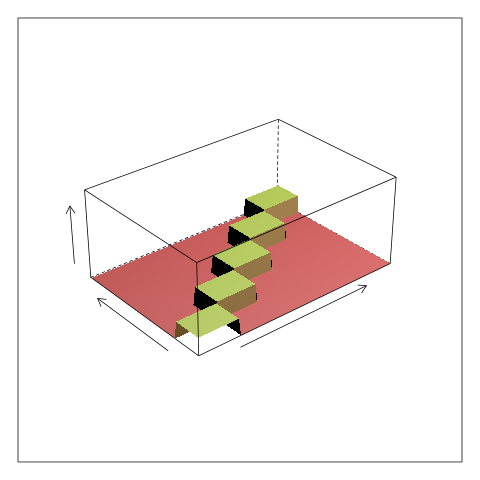
\includegraphics[width=.3\textwidth]{../FIGURES/CommunityTrueGraphon} &
  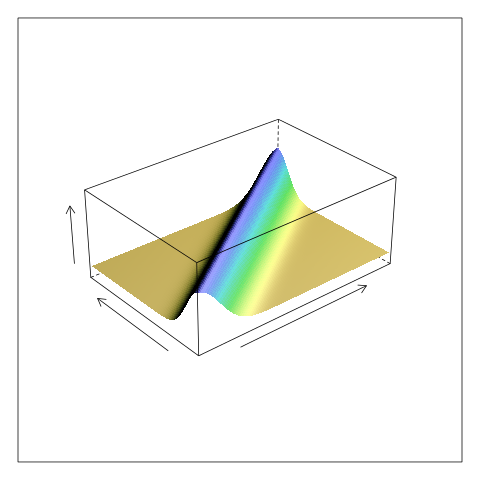
\includegraphics[width=.3\textwidth]{../FIGURES/SmallWorldTrueGraphon} 
  \end{tabular}
  } 
  
  \bigskip \pause
  \paragraph{Remark:} $\gamma(\cdot, \cdot) = $cst \ra ER model

}

%====================================================================
\frame{ \frametitle{Few words about the $W$-graph}

  \paragraph{Probabilistic point of view.}
  \begin{itemize}
   \item $W$-graph have been mostly studied in the probability literature: \refer{LoS06}, \refer{DiJ08}
   \item Motif (sub-graph) frequencies are invariant characteristics of a $W$-graph.
   \item Intrinsic un-identifiability of the graphon function $\gamma$ is often overcome by imposing that $u \mapsto \int \gamma(u, v) \dd v$ is monotonous increasing.
  \end{itemize}

  \bigskip \bigskip \pause
  \paragraph{Statistical point of view.}
  \begin{itemize}
   \item A series of works on the inference of the graphon: \refer{Kal99}, \refer{Hof08}, %\refer{BCL11},
   \refer{ACC13}, \refer{Cha14}, \refer{OlW14}, ...
   \item Many non-parametric approaches
   \item SBM sometimes used as a proxy for $W$-graph.
  \end{itemize}
}

% %====================================================================
% \subsection*{Present framework and goals}
% %====================================================================
% \frame{\frametitle{Present framework and goals}
% 
%   \paragraph{Parametric setting.}
%   \begin{itemize}
%    \item Use SBM as a proxy for the $W$-graph.
%    \item Use variational Bayes inference and model averaging to infer the graphon $\phi$
%   \end{itemize}
% 
%   \bigskip \bigskip 
%   \paragraph{Goodness-of-fit.}
%   \begin{itemize}
%    \item Assess the goodness-of-fit of the $W$-graph model
%   \end{itemize}
%   
%   \bigskip \bigskip
%   \paragraph{Covariates.}
%   \begin{itemize}
%    \item Account for the effect of (edge) covariates via a regression term
%    \item Assess the goodness-of-fit of the regression model.
%   \end{itemize}
% }

%====================================================================
%====================================================================
\section{Variational Bayes inference for SBM and $W$-graph}
\frame{\frametitle{Outline} \tableofcontents[currentsection]}
%====================================================================

%====================================================================
\subsection*{Variational Bayes inference for SBM}
%====================================================================
\frame{\frametitle{Variational inference for latent space graph models}

  \paragraph{Incomplete data model.} Latent space models for graphs are part of incomplete data model. 
  $$
  \text{\ra Need to deal with} \qquad P(Z|Y) \; \text{ or } \; P(Z|Y, \theta)
  $$

  \pause
  \paragraph{Conditional dependency.}  Because the graph structure of the data,
  $$
  P(Z|\theta) = \prod_i P(Z_i|\theta)
  \qquad \text{but} \qquad
  P(Z|\theta, Y) \neq \prod_i P(Z_i|\theta, Y)
  $$
  
  \pause
  \paragraph{Variational (Bayes) approximation \refer{WaJ08}.}  Need for an approximate distribution:
  $$
  \Pt_Y(Z, \theta) := \Pt_Y(\theta) \prod_i \Pt_Y(Z_i) \quad \approx \quad P(Z, \theta|Y).
  $$
  '$\approx$' means, e.g., minimal in terms of KL divergence:
  $$
  \Pt_Y(Z, \theta) = \arg\min_Q KL\left(\left.\left.Q(\theta) \prod_i Q(Z_i) \right|\right| P(Z, \theta|Y)\right).
  $$
  \pause
  \paragraph{Variational Bayes EM (VBEM) algorithm:} close form updates when using conjugate priors \refer{BeG03}.
}

%====================================================================
\frame{\frametitle{Properties of variational estimates for SBM}

  \begin{itemize}
   \item VEM and VBEM algorithms have been specifically developed for SBM: \refer{DPR08}, \refer{LBA11b}
%    \item Model selection (choice of $K$ has also be addressed): \Refer{same refs}.
   \item Theoretical justifications of the variational approximation exist for SBM in a frequentist setting: \refer{CDP12}, \refer{MaM14}.
   \item Only simulation-based arguments in the Bayesian setting.
  \end{itemize}

  \bigskip \pause
  \paragraph{Credibility intervals:}   $\pi_1$: $+$,
  $\gamma_{11}$: \textcolor{red}{$\triangle$}, $\gamma_{12}$:
  \textcolor{blue}{$\circ$}, $\gamma_{22}$: \textcolor{green}{$\bullet$} \\
%   $$
  \includegraphics[width=1\textwidth]{../FIGURES/im-ICQ2-2-new} \\
%   $$
%   \vspace{-.5\textheight}
  \pause
  \paragraph{Heuristic:} $P(Z|Y) \rightarrow \delta_{z^*}$ (the classification task is asymptotically trivial: \refer{CDR12}) and $\Pt(\theta|Y, Z) = P(\theta|Y, Z)$ thanks to conjugacy.
}

%====================================================================
\subsection*{Variational Bayes inference for $W$-graph}
%====================================================================
\frame{ \frametitle{SBM as a $W$-graph model}

  \begin{tabular}{cc}
    \hspace{-.02\textwidth}
    \begin{tabular}{p{.5\textwidth}}
	 Latent variables:
	 $$
	 (Z_i) \text{ iid } \sim \Mcal(1, \pi)
	 $$ ~\\
	 Blockwise constant graphon:
	 $$
	 \gamma(z, z') = \gamma_{k\ell}
	 $$ ~\\
	 Edges:
	 $$
	 \Pr\{Y_{ij} = 1\} = \gamma(Z_i, Z_j)
	 $$    
	 \end{tabular}
    & 
    \hspace{-.1\textwidth}
    \begin{tabular}{p{.5\textwidth}}
	 Graphon function $\gamma^{SBM}_K(z, z')$ \\
      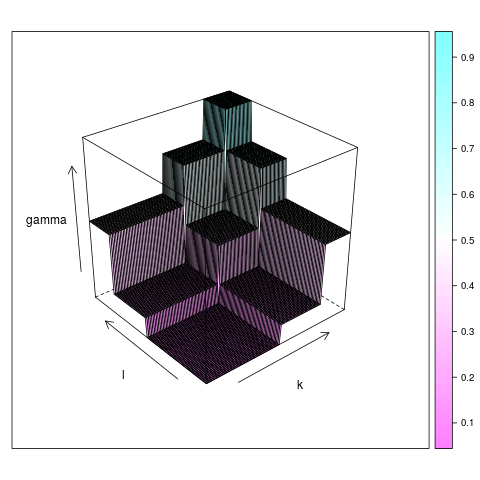
\includegraphics[width=.5\textwidth]{../FIGURES/FigCLADAG-SBM-graphon} \\
    \end{tabular}
  \end{tabular} 

  \ra block widths $= \pi_k$, block heights $\gamma_{k\ell}$
 }

%====================================================================
\frame{ \frametitle{Variational Bayes estimation of $\gamma(z, z')$}

  \begin{tabular}{cc}
    \hspace{-.02\textwidth}
    \begin{tabular}{p{.45\textwidth}}
    \paragraph{VBEM inference} provides the \\approximate posteriors:
    \begin{eqnarray*}
    (\pi | Y) & \approx & \text{Dir}(\pi^*) \\
    (\gamma_{k\ell} | Y) & \approx & \text{Beta}(\gamma^{0*}_{k\ell}, \gamma^{1*}_{k\ell}) 
    \end{eqnarray*}
    ~
    
    \bigskip 
    \paragraph{Estimate of $\gamma(u, v)$.} 
    Due \\
    to the uncertainty of the $\pi_k$, \\
    the posterior mean of $\gamma^{SBM}_K$  \\
    is smooth
    
    \bigskip 
    (Explicit integration using \refer{GoS10})
    \end{tabular}
    & 
    \hspace{-.05\textwidth}
    \begin{tabular}{p{.5\textwidth}}
	 Posterior mean $\widetilde{\Esp}(\gamma^{SBM}_K(z, z') | Y, K)$ \\
      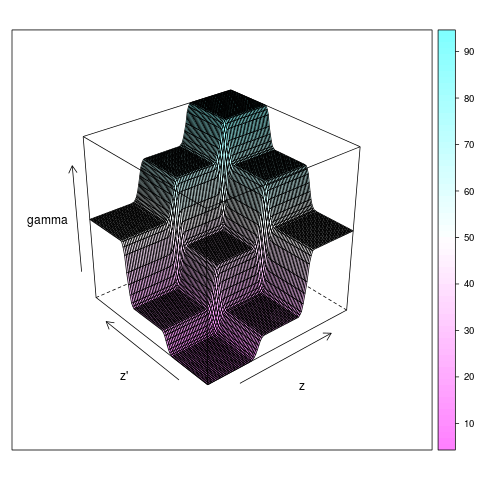
\includegraphics[width=.5\textwidth]{../FIGURES/FigGraphon-SBM-average} \\
    \end{tabular}
  \end{tabular}
  
}

%====================================================================
\frame{\frametitle{From SBM to $W$-graph: Averaging models}

  \paragraph{Bayesian model averaging (BMA).} Consider a series of SBM $1, \dots, K, \dots$, each with its respective graphon function $\gamma_K^{SBM}(z, z')$. We have that
  $$
  \Esp[\gamma(z, z') | Y] = \sum_K P(K|Y) \Esp[\gamma_K^{SBM}(z, z') | Y]
  $$

  \bigskip \pause
  \paragraph{Pushing the variational approximation further:} Consider the model $K$ as an additional hidden variable:
  $$
  P(Z, \theta, K|Y) \approx \Pt_Y(Z, \theta, K) 
  := \Pt_Y(Z|K) \times \Pt_Y(\theta|K) \times \Pt_Y(K)  
  $$
  
  \bigskip \pause
  \paragraph{Variational Bayes model averaging (VBMA).} The KL-optimal approximation of $P(K|Y)$ satisfies \refer{VMR12}: 
  $$
    \Pt_Y(K) \propto P(K) e^{\log P(Y|K) - KL(K)} = P(K|Y) e^{-\emphase{KL(K)}}
  $$ 
  where $KL(K) = KL[\Pt_Y(Z, \theta|K) \Vert P(Z,  \theta|Y, K)]$. 

}

%====================================================================
\frame{\frametitle{Inferring the graphon function}

  \paragraph{Model averaging:} There is no 'true $K$' in the $W$-graph model.

  \bigskip \bigskip \bigskip
  \paragraph{Apply VBMA recipe to $\gamma(z, z')$.}
  For $K = 1 .. K_{\max}$, fit an SBM model via VBEM and compute
  $$
  \widehat{\gamma}_K^{SBM}(z, z') = \widetilde{\Esp}[\gamma_{C(z), C(z')} | Y, K]
  $$
  where $C(z)$ stands for the SBM class at abscissa $z$.
  
  \pause \bigskip \bigskip \bigskip
  Then perform model averaging as
  $$
  \widehat{\gamma}(z, z') = \widetilde{\Esp}[\gamma_{C(z), C(z')} | Y] = \sum_K \Pt_Y(K) \widehat{\gamma}_K^{SBM}(z, z'),
  $$
  \Refer{Latouche and R. (2013)}\nocite{LaR13}.
%   \end{itemize}
}

%====================================================================
\subsection*{Some examples}
%====================================================================
\frame{\frametitle{Ecological network between fungal species}

  Link between 2 fungi if they are observed on one common host.

  \begin{tabular}{cc}
    \begin{tabular}{p{.5\textwidth}}
	 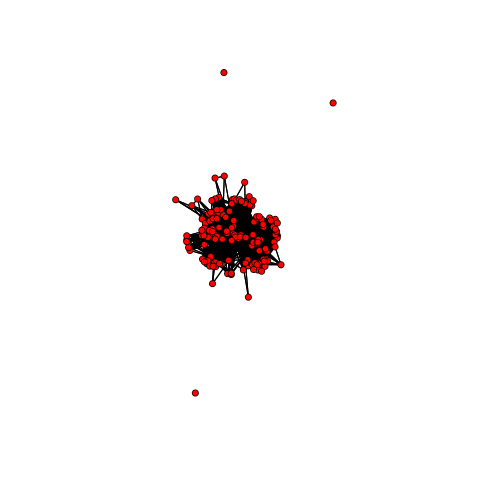
\includegraphics[width=.45\textwidth]{../FIGURES/Fungi-graph}
    \end{tabular}
    & 
    \hspace{-.1\textwidth}
    \begin{tabular}{p{.5\textwidth}}
	 \begin{overprint}
	 \onslide<1>
	 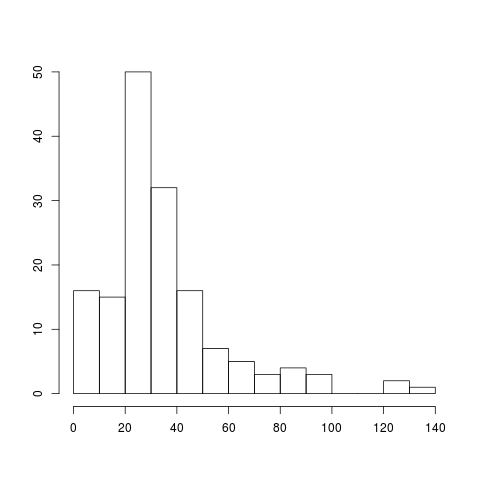
\includegraphics[width=.45\textwidth]{../FIGURES/Fungi-degree}
	 \onslide<2>
	 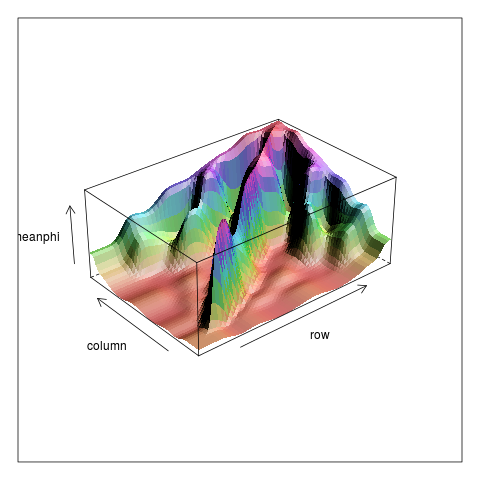
\includegraphics[width=.45\textwidth]{../FIGURES/Fungi-graphon}
	 \end{overprint}
    \end{tabular}
  \end{tabular}
}

%====================================================================
\frame{\frametitle{Brain network}

  Links = connexions between areas of the macaque's cortex

  \begin{tabular}{cc}
    \begin{tabular}{p{.5\textwidth}}
	 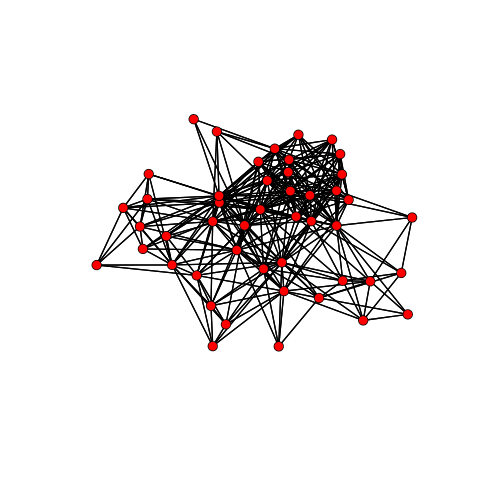
\includegraphics[width=.45\textwidth]{../FIGURES/Macaque-graph}
    \end{tabular}
    & 
    \hspace{-.1\textwidth}
    \begin{tabular}{p{.5\textwidth}}
	 \begin{overprint}
	 \onslide<1>
	 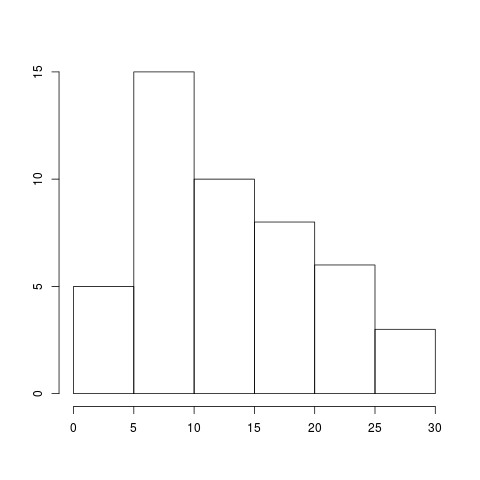
\includegraphics[width=.45\textwidth]{../FIGURES/Macaque-degree}
	 \onslide<2>
	 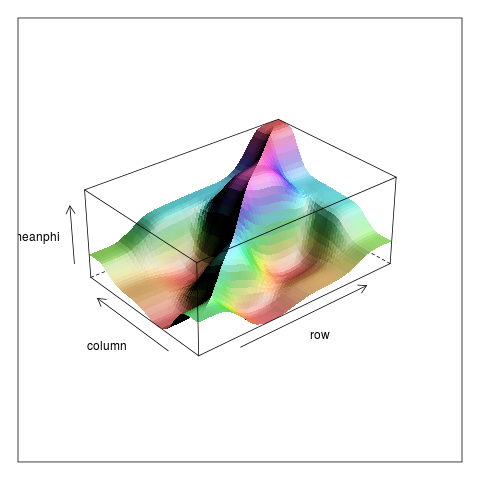
\includegraphics[width=.45\textwidth]{../FIGURES/Macaque-graphon}
	 \end{overprint}
    \end{tabular}
  \end{tabular}
}

%====================================================================
\frame{\frametitle{Blog network}

  Links = connexions between French political blogs

  \begin{tabular}{cc}
    \begin{tabular}{p{.5\textwidth}}
	 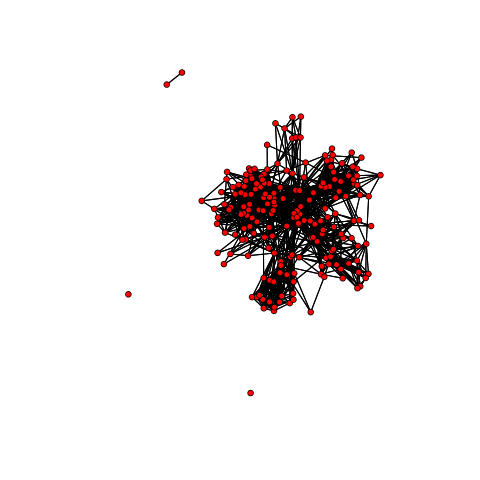
\includegraphics[width=.45\textwidth]{../FIGURES/Blog-graph}
    \end{tabular}
    & 
    \hspace{-.1\textwidth}
    \begin{tabular}{p{.5\textwidth}}
	 \begin{overprint}
	 \onslide<1>
	 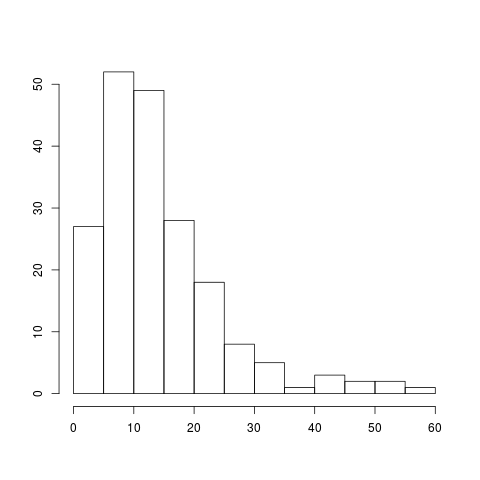
\includegraphics[width=.45\textwidth]{../FIGURES/Blog-degree}
	 \onslide<2>
	 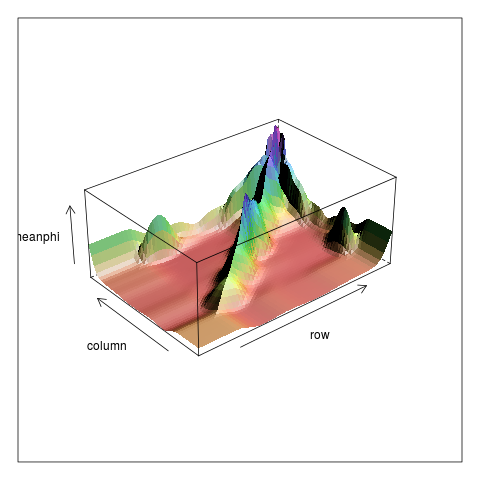
\includegraphics[width=.45\textwidth]{../FIGURES/Blog-graphon}
	 \end{overprint}
    \end{tabular}
  \end{tabular}
}

%====================================================================
%====================================================================
\section{Goodness of fit}
\frame{\frametitle{Outline} \tableofcontents[currentsection]}
%====================================================================

%====================================================================
\subsection*{Motifs frequency}
%====================================================================
\frame{\frametitle{Motifs frequency}

  \vspace{-0.1\textheight}
  $$
  \begin{tabular}{cccccc}
  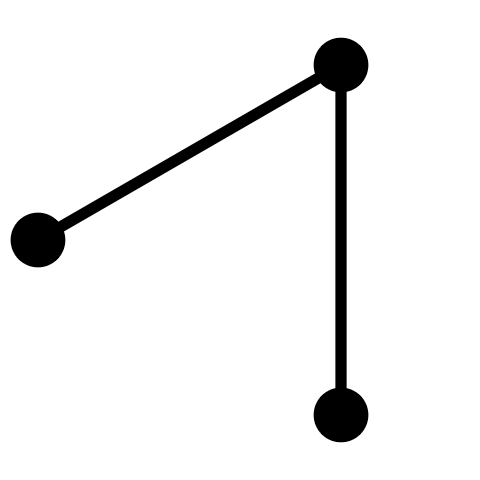
\includegraphics[width=.1\textwidth]{../FIGURES/FigMotif-V}
  & 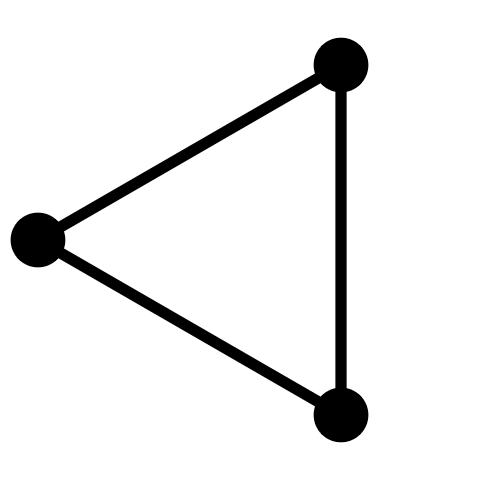
\includegraphics[width=.1\textwidth]{../FIGURES/FigMotif-Triangle}
  & 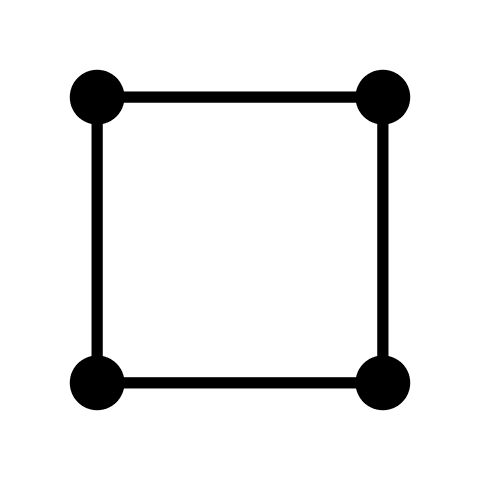
\includegraphics[width=.1\textwidth]{../FIGURES/FigMotif-Square}
  & 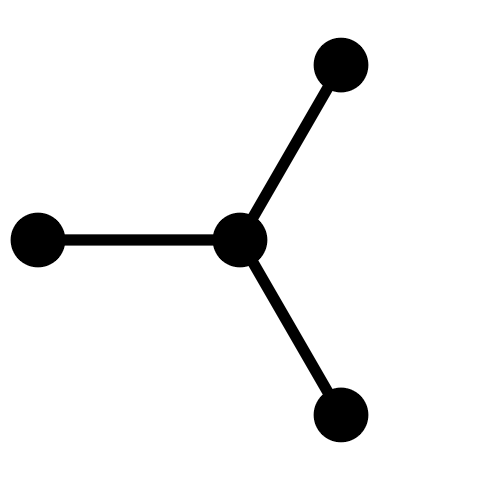
\includegraphics[width=.1\textwidth]{../FIGURES/FigMotif-Star3}
  & 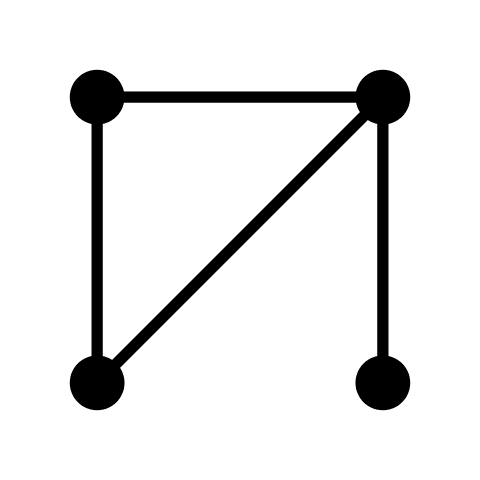
\includegraphics[width=.1\textwidth]{../FIGURES/FigMotif-Whisker}
  & 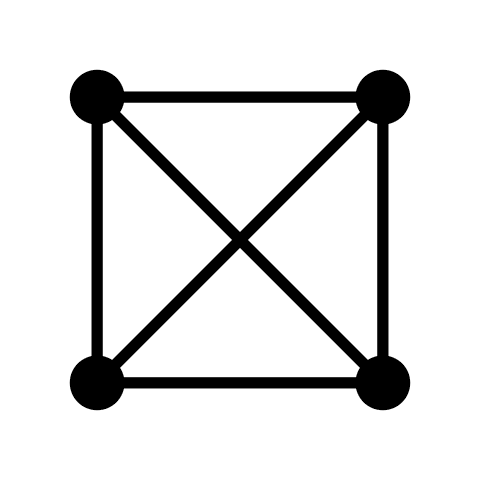
\includegraphics[width=.1\textwidth]{../FIGURES/FigMotif-Clique4}
  \end{tabular}
  $$
  
  \begin{itemize}
  \item Network motifs have a biological or sociological interpretation in terms of building blocks of the global network \\
  \ra Triangles = 'friends of my friends are my friends'. \\ ~
  \item Latent space graph models only describe binary interactions, conditional on the latent positions
  \end{itemize} 
  
  \bigskip
  \ra Goodness of fit criterion based on motif frequencies?
    
}

%====================================================================
\frame{\frametitle{Moments of motif counts}

  \paragraph{Moments under SBM:} The first moments $\Esp N(m)$, $\Var N (m)$ of the count are known for exchangeable graph models (incl. SBM) \refer{PDK08}: 
  $$
  \Esp_{SBM} N(m) \propto  \mu_{SBM}(m) =: f(\theta_{SBM}) %, \Var_{SBM(K)} N(m)
  $$
  where $\mu_{SBM}(m)$ is the motif occurrence probability under SBM.
  
  \bigskip \bigskip 
  \paragraph{Moments under $W$-graph:} Motif probability under the $W$ -graph can be estimated as 
  $$
  \widehat{\mu}(m) = \sum_k \Pt(K) \widetilde{\Esp}(\mu_{SBM}(m) | X, K)
  $$
  Estimates of $\Esp_W N(m)$ and $\Var_W N(m)$ can be derived accordingly   \Refer{Latouche and R. (2013)}\nocite{LaR13}.
    
}

%====================================================================
\frame{ \frametitle{Network frequencies in the blog network}

\vspace{-0.1\textheight}
$$
\begin{tabular}{crrrr}
  \hline
 Motif & Count & Mean & Std. dev. \\ % & approx $p$-value \\ 
 & ($\times 10^3$) & ($\times 10^3$) & ($\times 10^3$) \\ % & \refer{PDK08} \\ 
  \hline
  \begin{tabular}{c} 
\includegraphics[width=.045\textwidth]{../FIGURES/FigMotif-I} \end{tabular} & 29.7 & 39.7 & 8.3 \\ % & 0.89 \\ 
  \begin{tabular}{c} 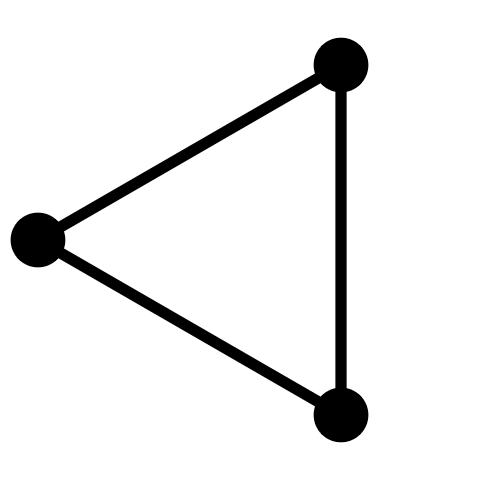
\includegraphics[width=.045\textwidth]{../FIGURES/FigMotif-Triangle} \end{tabular} & 3.8 & 4.6 & 1.3 \\ % & 0.69 \\ 
  \begin{tabular}{c} 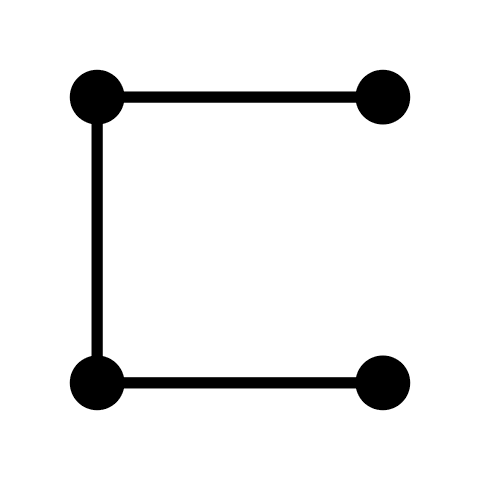
\includegraphics[width=.045\textwidth]{../FIGURES/FigMotif-Chain4} \end{tabular} & 608.7 & 968.3 & 336.8 \\ % & 0.86 \\ 
  \begin{tabular}{c} 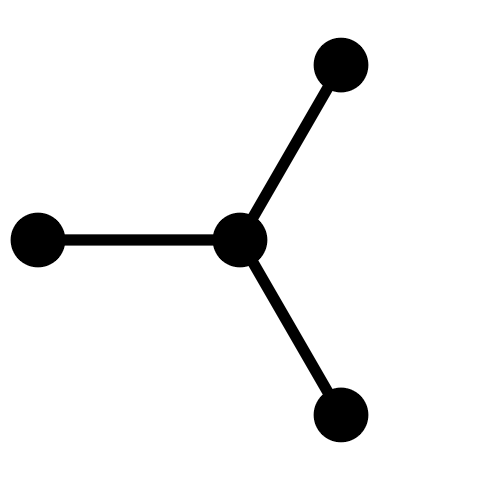
\includegraphics[width=.045\textwidth]{../FIGURES/FigMotif-Star3} \end{tabular}  & 279.8 & 428.9 & 154.0 \\ % & 0.83 \\ 
  \begin{tabular}{c} 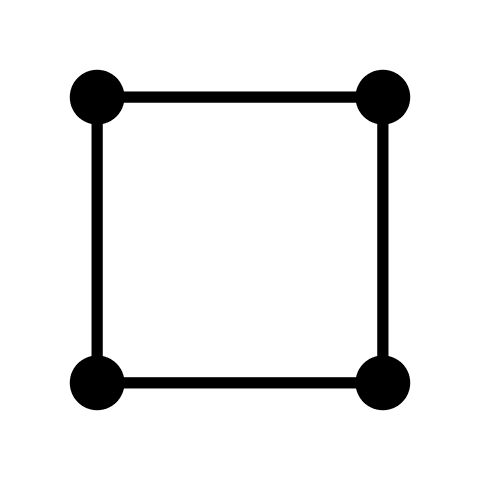
\includegraphics[width=.045\textwidth]{../FIGURES/FigMotif-Square} \end{tabular} & 47.4 & 74.5 & 35.1 \\ % & 0.77 \\ 
  \begin{tabular}{c} 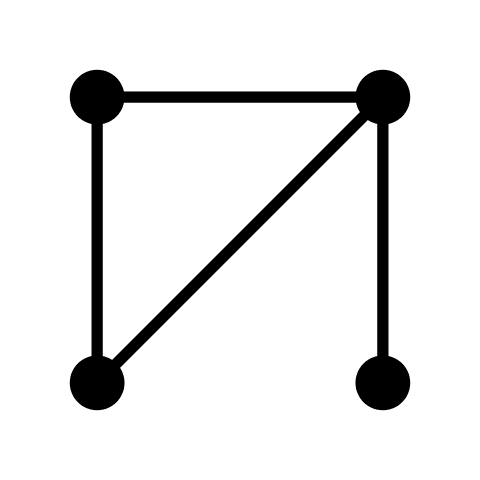
\includegraphics[width=.045\textwidth]{../FIGURES/FigMotif-Whisker} \end{tabular} & 270.5 & 397.0 & 177.0 \\ % & 0.75 \\ 
  \begin{tabular}{c} 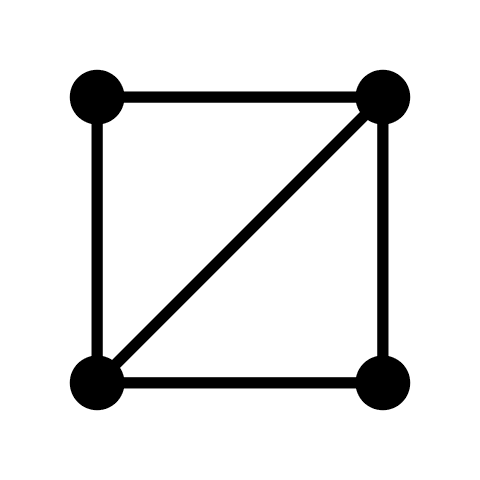
\includegraphics[width=.045\textwidth]{../FIGURES/FigMotif-SquareDiag} \end{tabular} & 62.1 & 87.8 & 47.4 \\ % & 0.67 \\ 
  \begin{tabular}{c} 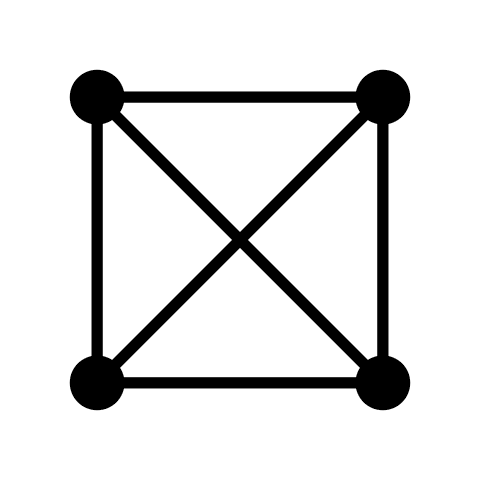
\includegraphics[width=.045\textwidth]{../FIGURES/FigMotif-Clique4} \end{tabular} & 6.5 & 8.8 & 5.4 \\ % & 0.61 \\ 
   \hline
\end{tabular}
$$

No specific structure seems to be exceptional wrt the model's expectations.

}

%====================================================================
\subsection*{Introducing covariates}
%====================================================================
\frame{\frametitle{Adding covariates: re-parametrization}

  \paragraph{SBM without covariate: re-parametrization} 
  \begin{itemize}
   \item Regular SBM parametrization:
   $$
   P(Y_{ij} = 1 | Z, \gamma) = \gamma_{Z_i, Z_j}
   $$
   \item \pause Logit transform: $\logit \; \gamma = [\logit \; \gamma_{k\ell}]$
   $$
   \logit \; P(Y_{ij} = 1 | Z, \gamma) = (\logit \; \gamma)_{Z_i, Z_j}.
   $$
  \end{itemize} \pause
  \ra Same probabilistic model, but different Bayesian setting:
  $$
  \begin{array}{rcrclcl}
  \text{prior:} & & \gamma_{k\ell} & \sim & \Beta(\cdot ,\cdot) & & \text{\ra conjugacy}, \\
  \\
  \text{prior:} & & \logit \; \gamma_{k\ell} & \sim & \Ncal(\cdot, \cdot) & & \text{\ra no conjugacy}
  \end{array}
  $$
%   A VB-EM can still be designed \refer{JaJ00}.
  
  \bigskip \bigskip \pause
  \paragraph{$W$ graph.} The same logit transform applies:
  $$
  P(Y_{ij} = 1 | Z, \gamma) = \gamma(Z_i, Z_j)
  \quad \rightarrow \quad
  \logit \; P(Y_{ij} = 1 | Z, \gamma) = \logit \; \gamma(Z_i, Z_j).
  $$
}

%====================================================================
\frame{\frametitle{Adding covariates: GLM framework}

  \paragraph{SBM:} Adding edge covariates is easy in the generalized linear model framework \refer{MRV10}:
  $$
  \logit \; P(Y_{ij} = 1 | Z, \beta) = x_{ij} \beta + \logit \; \gamma_{Z_i, Z_j}.
  $$
  \ra A VB-EM algorithm can be designed as well using \refer{JaJ00}. 
  
  
  \pause \bigskip
  \paragraph{$W$-graph:} Works the same :
  $$
  \logit \; P(Y_{ij} = 1 | Z, \beta) = x_{ij} \beta + \logit \; \gamma(Z_i, Z_j)
  $$
  \ra $\gamma(Z_i, Z_j)$ can be interpreted as a 'residual' graphon.

  \bigskip \bigskip \pause
  \paragraph{Goodness-of-fit.} Whenever the covariates suffice to explain the heterogeneity of the graph: $\Esp[\gamma(z, z')|Y]$ should be flat, that is
  $$
  P(K=1 | Y) \simeq 1.
  $$
  }

%====================================================================
\subsection*{Residual graphon}
%====================================================================
\frame{ \frametitle{Tree network}

\newcommand{\GOFplot}{/home/robin/Dropbox/vbemapp/GOF2/code_gof/plot}

  \begin{tabular}{cc}
    \begin{tabular}{p{.5\textwidth}}
    \onslide+<1->{\paragraph{Binary version:} 
    Links between tree species if they host at least one common fungal parasite. 
    $$
    \arg\max_K \Pt(K|Y) = 9
    $$\\}
    \onslide+<2>{\paragraph{Regression:}
    covariates = genetic distance, taxonomic distance, geographic distance
    $$
    \arg\max_K \Pt(K|Y) = 3
    $$}
    \end{tabular}
    & 
    \hspace{-.05\textwidth}
    \begin{tabular}{p{.5\textwidth}}
    \begin{overprint}
     \onslide<1>
     \includegraphics[width=.45\textwidth]{\GOFplot/tree_nocovariates}
     \onslide<2>
     \includegraphics[width=.45\textwidth]{\GOFplot/tree_3covariates}
    \end{overprint}
    \end{tabular}
  \end{tabular}
  
    \onslide+<2>{\ra The residual graphon is not flat: some heterogeneity remains.}
  
}

%====================================================================
\frame{ \frametitle{Blog network}

  \newcommand{\GOFplot}{/home/robin/Dropbox/vbemapp/GOF2/code_gof/plot}
  
  \begin{tabular}{cc}
    \begin{tabular}{p{.5\textwidth}}
    \onslide+<1->{\paragraph{Blog network:} 
    Already shown. 
    $$
    \arg\max_K \Pt(K|Y) = 12
    $$\\}
    \onslide+<2>{\paragraph{Regression:}
    covariates = same political party, pair includes a journalist
    $$
    \arg\max_K \Pt(K|Y) = 5
    $$}
    \end{tabular}
    & 
    \hspace{-.15\textwidth}
    \begin{tabular}{p{.5\textwidth}}
    \begin{overprint}
     \onslide<1>
     \hspace{-.05\textwidth}
     \includegraphics[width=.7\textwidth, clip=]{\GOFplot/blog_nocovariates}
     \onslide<2>
     \includegraphics[width=.6\textwidth]{\GOFplot/blog_2covariates}
    \end{overprint}
    \end{tabular}
  \end{tabular}

    \onslide+<2>{\ra The residual graphon is still not flat.}
}

%====================================================================
\section*{Conclusion}
\frame{ \frametitle{Conclusion \& future work}

  \paragraph{Some conclusions.}
  \begin{itemize}
   \item The graphon provides a representation of the network topology
   \item It can be estimated using variational Bayes inference \\
   \ra R packages 'mixer' and 'blockmodels'
   \item It can be combined with covariates as a residual term
  \end{itemize}
  
  \bigskip \bigskip \pause
  \paragraph{Future (on-going) work.}
  \begin{itemize}
   \item Formal goodness-of-fit test
   \item Quality of variational Bayes estimates in SBM with covariates
  \end{itemize}

%   \bigskip \bigskip 
%   Thank you for your attention.

}

%====================================================================
\frame[allowframebreaks]{ \frametitle{References}
{\tiny
  \bibliography{/home/robin/Biblio/ARC,/home/robin/Biblio/AST}
  \bibliographystyle{/home/robin/LATEX/Biblio/astats}
  %\bibliographystyle{plain}
  }
}
%====================================================================
\frame{\frametitle{VBEM inference for SBM: {\sl E. coli}'s operon network}

  \vspace{-0.5cm}
  \hspace{-0.5cm}
  \begin{tabular}{cc}         
    \begin{tabular}{p{0.45\textwidth}}
%     \begin{overprint}
       \onslide<1->{
       \vspace{-1cm}
       \includegraphics[width=.45\textwidth]{\fignet/im_EcoliVEM_2} \\
       %~\\
       \refer{PMD09}
       }
%     \end{overprint}
    \end{tabular}
    &
    \begin{tabular}{p{0.45\textwidth}}
     \onslide+<2->{
      \vspace{-.3cm}
      \paragraph{Meta-graph representation.} \\
      %\vspace{-.02\textwidth}
      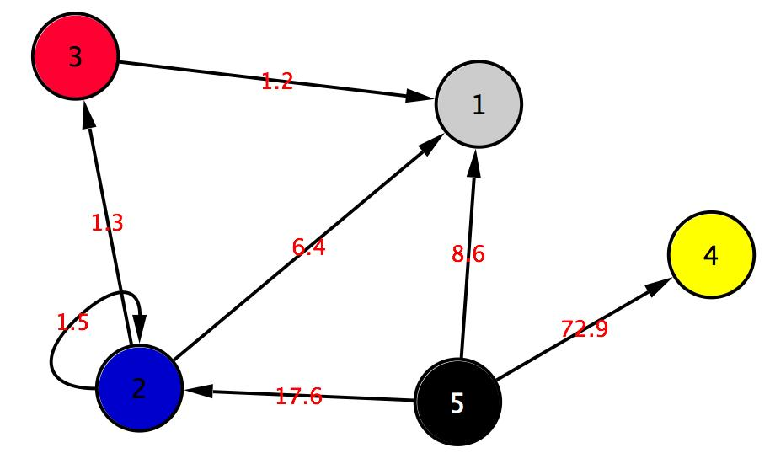
\includegraphics[width=.35\textwidth]{\fignet/VEMmetagraphe}  \\
     }
     \onslide+<3->{
      \vspace{-.3cm}
      \paragraph{Parameter estimates.} $K = 5$     \\
      \includegraphics[width=.35\textwidth]{../FIGURES/im-pi1BVEM}\\        
      \includegraphics[width=.35\textwidth]{../FIGURES/im-pi2BVEM}\\
      \includegraphics[width=.35\textwidth]{../FIGURES/im-pi3BVEM}\\
      \includegraphics[width=.35\textwidth]{../FIGURES/im-pi4BVEM}\\
      \includegraphics[width=.35\textwidth]{../FIGURES/im-pi5BVEM}\\
      \hline 
      \includegraphics[width=.35\textwidth]{../FIGURES/im-alphaBVEM}\\
     }
    \end{tabular}
  \end{tabular}
  }

%====================================================================
%====================================================================
\end{document}
%====================================================================
%====================================================================

  \begin{tabular}{cc}
    \begin{tabular}{p{.5\textwidth}}
    \end{tabular}
    & 
    \hspace{-.02\textwidth}
    \begin{tabular}{p{.5\textwidth}}
    \end{tabular}
  \end{tabular}

